\documentclass{standalone}
\usepackage[centertags]{amsmath}
\usepackage{latexsym}
\usepackage{amsfonts}
\usepackage{amssymb}
\usepackage{amsthm}
\usepackage{newlfont}
\usepackage{enumerate}
\usepackage{makeidx}
\usepackage{tikz}
\usepackage{nicematrix}

\usetikzlibrary{matrix,fit,positioning,arrows.meta}

\begin{document}
    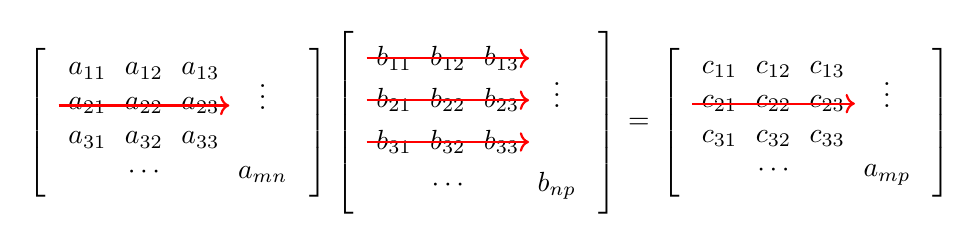
\begin{tikzpicture}
   \matrix (A) [matrix of math nodes,left delimiter=\lbrack,right delimiter=\rbrack]
{
a_{11} & a_{12} & a_{13} & \ \\
a_{21} & a_{22} & a_{23}  & \smash{\vdots} \\
a_{31} & a_{32} & a_{33} &  \\
& \cdots & \ & a_{mn} \\
};
   \matrix (B) [matrix of math nodes,left delimiter=\lbrack,right delimiter=\rbrack,xshift=-1em,right = of A]
{
b_{11} & b_{12} & b_{13} & \ \\
b_{21} & b_{22} & b_{23} & \smash{\vdots} \\
b_{31} & b_{32} & b_{33} & \\
& \cdots & \ & b_{np} \\
};
\node(eq)[right= of B,xshift=-2em]{=};
   \matrix (C) [matrix of math nodes,left delimiter=\lbrack,right delimiter=\rbrack,xshift=-2em,right = of eq]
{
c_{11} & c_{12} & c_{13} \\
c_{21} & c_{22} & c_{23} & \smash{\vdots} \\
c_{31} & c_{32} & c_{33} \\
& \cdots && a_{mp} \\ 
};
\draw[thick,red,->] (A-2-1.west) -- (A-2-3.east); 
\draw[thick,red,->] (B-1-1.west) -- (B-1-3.east); 
\draw[thick,red,->] (B-2-1.west) -- (B-2-3.east); 
\draw[thick,red,->] (B-3-1.west) -- (B-3-3.east);
\draw[thick,red,->] (C-2-1.west) -- (C-2-3.east); 

    \end{tikzpicture}
\end{document}
